\documentclass{article}

\usepackage{pgfplots}

\pgfplotsset{compat=1.11}

% \usetikzlibrary{}
% \usepgfplotslibrary{}



\begin{document}

Expectation: all produce the same picture

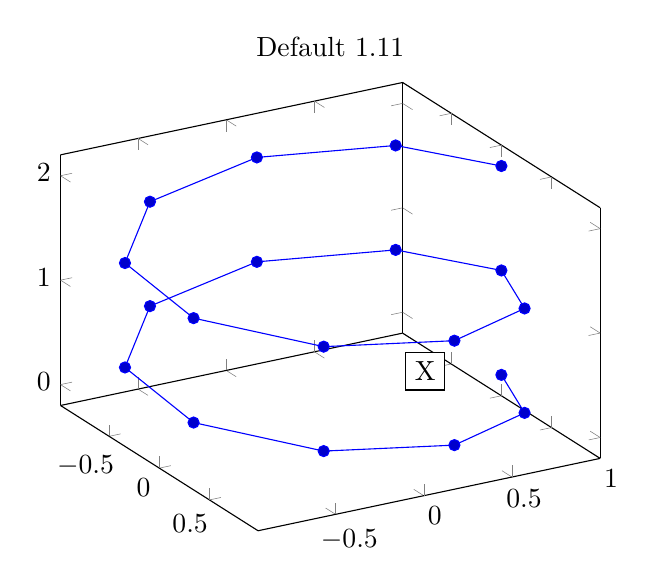
\begin{tikzpicture}
    \begin{axis}[view={60}{30},title=Default 1.11]
    \addplot3+[domain=0:2*360,samples=19,samples y=0]
        ({sin(x)},
         {cos(x)},
         {2*x/(2*360)});
	
	\node[fill=white,draw=black,anchor=center] at ({sin(90)},{cos(90)},1) {X};
    \end{axis}
\end{tikzpicture}
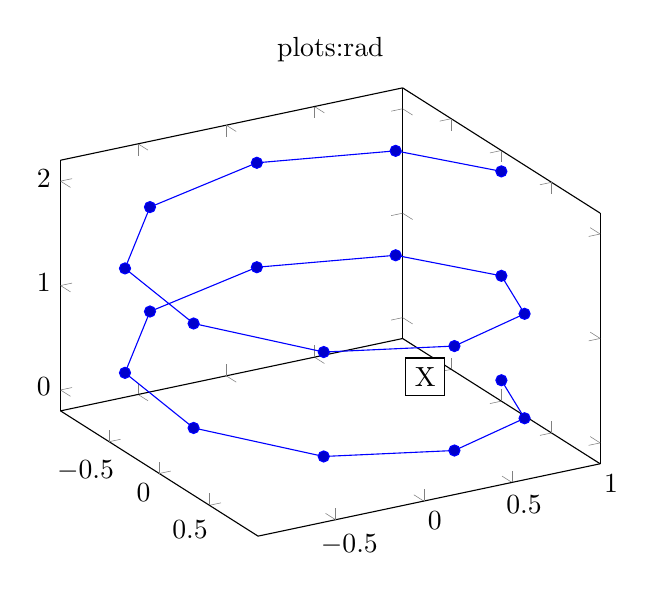
\begin{tikzpicture}
    \begin{axis}[view={60}{30},trig format plots=rad,title=plots:rad]
    \addplot3+[domain=0:4*pi,samples=19,samples y=0]
        ({sin(x)},
         {cos(x)},
         {2*x/(4*pi)});
	
	\node[fill=white,draw=black,anchor=center] at ({sin(90)},{cos(90)},1) {X};
    \end{axis}
\end{tikzpicture}

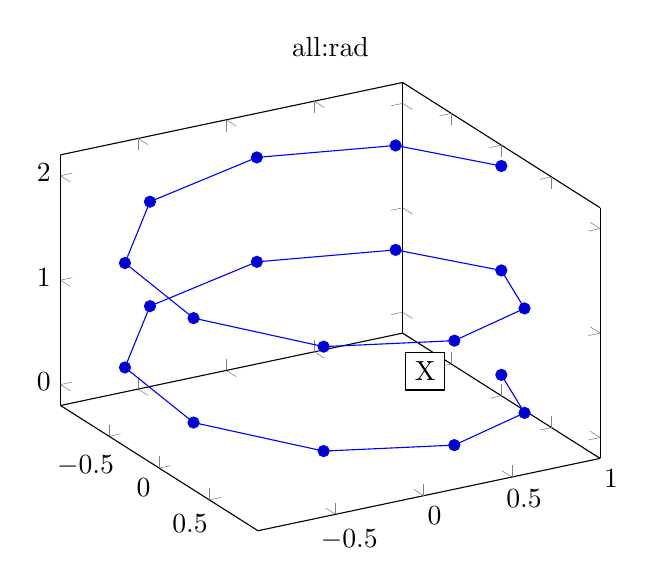
\begin{tikzpicture}
    \begin{axis}[view={rad(60)}{rad(30)},trig format=rad,title=all:rad]
    \addplot3+[domain=0:4*pi,samples=19,samples y=0]
        ({sin(x)},
         {cos(x)},
         {2*x/(4*pi)});
	
	\node[fill=white,draw=black,anchor=center] at ({sin(pi/2)},{cos(pi/2)},1) {X};
    \end{axis}
\end{tikzpicture}
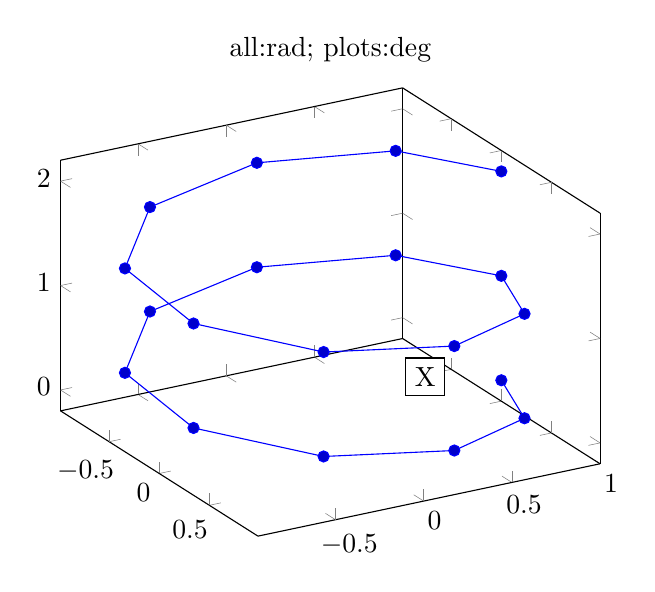
\begin{tikzpicture}
    \begin{axis}[view={rad(60)}{rad(30)},trig format=rad,trig format plots=deg,title=all:rad; plots:deg]
    \addplot3+[domain=0:2*360,samples=19,samples y=0]
        ({sin(x)},
         {cos(x)},
         {2*x/(2*360)});
	
	\node[fill=white,draw=black,anchor=center] at ({sin(pi/2)},{cos(pi/2)},1) {X};
    \end{axis}
\end{tikzpicture}


\end{document}

